\documentclass[english,t]{beamer}
%\documentclass[finnish,english,handout]{beamer}

% Uncomment if want to show notes
% \setbeameroption{show notes}

\mode<presentation>
{
  \usetheme{Warsaw}
  % oder ...
  
  \setbeamercovered{invisible}
  % oder auch nicht
}

% ==============================
%  Added Package
% ==============================
\usepackage[linesnumbered,lined,commentsnumbered]{algorithm2e}
\usepackage{bm}

% =======================================
%   Using symbols for a checklist
% =======================================
\usepackage{pifont}% http://ctan.org/pkg/pifont
\newcommand{\cmark}{\ding{51}}%
\newcommand{\xmark}{\ding{55}}%

% ======================================
%     No Figure in the caption
% ======================================
\setbeamertemplate{caption}{\insertcaption} %---> does not work
%\captionsetup{labelformat=empty,labelsep=none} % ---> it works

% ===================================================
\usepackage{graphicx}
\graphicspath{{./figs/}}
\usepackage[T1]{fontenc}
\usepackage[latin1]{inputenc}
\usepackage{times}
\usepackage{epic,epsfig}
\usepackage{subfigure,float}
\usepackage{amsmath,amsfonts,amssymb}
\usepackage{inputenc}
\usepackage{babel}
\usepackage{afterpage}
\usepackage{eufrak}
\usepackage{amsbsy}
\usepackage{eucal}
\usepackage{rotating}
\usepackage{url}
\urlstyle{same}

\usepackage{natbib}
\bibliographystyle{apalike}

% \definecolor{hutblue}{rgb}{0,0.2549,0.6784}
% \definecolor{midnightblue}{rgb}{0.0977,0.0977,0.4375}
% \definecolor{hutsilver}{rgb}{0.4863,0.4784,0.4784}
% \definecolor{lightgray}{rgb}{0.95,0.95,0.95}
% \definecolor{section}{rgb}{0,0.2549,0.6784}
% \definecolor{list1}{rgb}{0,0.2549,0.6784}
 \definecolor{navyblue}{rgb}{0,0,0.5}
\renewcommand{\emph}[1]{\textcolor{navyblue}{#1}}

% \graphicspath{./pics}

\pdfinfo{            
  /Title      (Bayesian data analysis 2) 
  /Author     (Aki Vehtari) % 
  /Keywords   (Bayesian probability theory, Bayesian inference, Bayesian data analysis)
}


\parindent=0pt
\parskip=8pt
\tolerance=9000
\abovedisplayshortskip=0pt

\setbeamertemplate{navigation symbols}{}
\setbeamertemplate{headline}[default]{}
\setbeamertemplate{headline}[text line]{\insertsection}
\setbeamertemplate{footline}[frame number]


\def\o{{\mathbf o}}
\def\t{{\mathbf \theta}}
\def\w{{\mathbf w}}
\def\x{{\mathbf x}}
\def\y{{\mathbf y}}
\def\z{{\mathbf z}}

\DeclareMathOperator{\E}{E}
\DeclareMathOperator{\Var}{Var}
\DeclareMathOperator{\var}{var}
\DeclareMathOperator{\Sd}{Sd}
\DeclareMathOperator{\sd}{sd}
\DeclareMathOperator{\Gammad}{Gamma}
\DeclareMathOperator{\Invgamma}{Inv-gamma}
\DeclareMathOperator{\Bin}{Bin}
\DeclareMathOperator{\Negbin}{Neg-bin}
\DeclareMathOperator{\Poisson}{Poisson}
\DeclareMathOperator{\Beta}{Beta}
\DeclareMathOperator{\logit}{logit}
\DeclareMathOperator{\N}{N}
\DeclareMathOperator{\U}{U}
\DeclareMathOperator{\BF}{BF}
\DeclareMathOperator{\Invchi2}{Inv-\chi^2}
% \DeclareMathOperator{\Pr}{Pr}
\def\euro{{\footnotesize \EUR\, }}
\DeclareMathOperator{\rep}{\mathrm{rep}}


% ============
% Otsikko sivu
% ============

\title[]{Teori \& Soal KSNP 2020}
\subtitle{}

\author{Hendra Bunyamin}

\institute[  Maranatha]
{
  Teknik Informatika \\
  Fakultas Teknologi Informasi \\
  Universitas Kristen Maranatha
}

\date[NUNI IT Online] % (optional, should be abbreviation of conference name)
{26 Mei 2021}

%\pgfdeclareimage[height=1.5cm]{university-logo}{images/logo-mcu}
%\logo{\pgfuseimage{university-logo}}

\begin{document} 

\begin{frame}
  \titlepage
\end{frame}

 \begin{frame}

   \frametitle{Outline dari Sesi ke-4}
  \begin{itemize}
\item Soal 1: Aritmetika Modular 
\item Soal 2: Himpunan
\item Soal 3: Logika
\item Soal 4: Masih Logika
\item Soal 5: Logika Terus?
\bigskip
\item Soal 6: Luas Bidang Datar
\item Soal 7: Jarak Terpendek
\item Soal 8: Kombinasi Berulang
\item Soal 9: Relasi Rekursif
\item Soal 10: \textit{Dynamic Programming}
\end{itemize}
\end{frame}

%%%%
\begin{frame}{Aritmatika Modular (1/2)}
	\begin{itemize}
		\item<2-> \textbf{Modulo} adalah suatu operator matematika untuk mendapatkan sisa bagi suatu bilangan terhadap suatu bilangan lainnya~\citep{aji2011pemrograman}.
		\item<3-> Operasi modulo bisa dilambangkan dengan \texttt{mod} pada bahasa Pascal atau \% pada bahasa C/C++ atau Java.
		\item<4-> Operasi $a$ mod $m$ biasa dibaca "$a$ modulo $m$", dan memberikan sisa hasil bagi $a$ oleh $m$.
		\item<5-> Contoh:
		\begin{itemize}
			\item<6-> 5 mod 3 = 2 \\
			\item<7-> 10 mod 2 = 0 \\
			\item<8-> 21 mod 6 = 3.
		\end{itemize}		
	\end{itemize}
\end{frame}

\begin{frame}{Aritmatika Modular (2/2)}
	Sifat-sifat dasar dari operasi modulo adalah
	\begin{itemize}   
		\item<2-> $(a+b) \mod m = ((a \mod m) + (b \mod m)) \mod m$
		\item<3-> $(a-b) \mod m = ((a \mod m) - (b \mod m)) \mod m$
		\item<4-> $(a \times b) \mod m = ((a \mod m) \times (b \mod m)) \mod m$
		\item<5-> $a^b \mod m = ((a \mod m)^b \mod m$
		\item<6-> $(-a) \mod m = (-(a \mod m) + m) \mod m$
	\end{itemize}
	
\onslide<7->{Sebagai contoh, Anda diberikan bilangan $n$ dan $k$, lalu diminta menghitung hasil $n! \mod k$.} \\
\onslide<8->{Pada contoh ini, $n! = n \times (n - 1) \times (n - 2) \times \ldots \times 1$.} \\
\onslide<9-> Seandainya kita menghitung $n!$ terlebih dahulu, kemudian baru dimodulo $k$, kemungkinan besar kita akan mendapatkan \textit{integer overflow}.	
\end{frame}

%
%\begin{frame}{Hello World!}
%\begin{algorithm}[H]
%	\SetKwData{Left}{left}
%	\SetKwData{This}{this}
%	\SetKwData{Up}{up}
%	\SetKwFunction{Union}{Union}
%	\SetKwFunction{FindCompress}{FindCompress}
%	\SetKwInOut{Input}{Input}
%	\SetKwInOut{Output}{Output}
%
%\Input{Suatu bil$Im$ of size $w\times l$ \\ and $n$}
%\Output{A partition of the bitmap}
%\BlankLine   
%\emph{special treatment of the first line}\;
%\For{$i\leftarrow 2$ \KwTo $l$}{
%	\emph{special treatment of the first element of line $i$}\;
%	\For{$j\leftarrow 2$ \KwTo $w$}{\label{forins}
%	\Left$\leftarrow$ \FindCompress{$Im[i,j-1]$}\;
%	\Up$\leftarrow$ \FindCompress{$Im[i-1,]$}\;
%	\This$\leftarrow$ \FindCompress{$Im[i,j]$}\;            
%	\If(\tcp*[h]{O(\Left,\This)==1}){\Left compatible with \This}{\label{lt}
%		\lIf{\Left $<$ \This}{\Union{\Left,\This}}
%		\lElse{\Union{\This,\Left}}
%	}
%	\If(\tcp*[f]{O(\Up,\This)==1}){\Up compatible with \This}{\label{ut}
%		\lIf{\Up $<$ \This}{\Union{\Up,\This}}
%		\tcp{\This is put under \Up to keep tree as flat as possible}\label{cmt}
%		\lElse{\Union{\This,\Up}}\tcp*[h]{\This linked to \Up}\label{lelse}
%		}
%	}   
%	\lForEach{element $e$ of the line $i$}{\FindCompress{p}}
%	}
%	\caption{disjoint decomposition}\label{algo_disjdecomp} 
%\end{algorithm}
%\end{frame}

\begin{frame}
  \frametitle{Soal 1: Aritmatika Modular} 
Diberikan sebuah barisan, $1, 4, 5, 16, 17, 20, 21, \ldots$, yang terurut menaik dan terbentuk dari bilangan $4$ pangkat atau penjumlahan dari bilangan $4$ pangkat yang berbeda (contoh: $4^0, 4^1, 4^1 + 4^0, 4^2, 4^2 + 4^0, \ldots$).

\textbf{Tentukan bilangan ke-$\bm{2020}$ yang dimodulo dengan $\bm{31}$}.
%   \begin{center}
%   \only<2>{\includegraphics[width=9cm]{dbinom1.pdf}}
%   \only<3>{\includegraphics[width=9cm]{dbinom10.pdf}}
%   \only<4>{\includegraphics[width=9cm]{dbinom10b.pdf}}
% \end{center}
\end{frame}


\begin{frame}
  \frametitle{Solusi (1/3)}

\begin{table}[!ht]
	\centering
	\begin{tabular}{|c|c|c|}
		\hline
		\multicolumn{1}{|c}{\textbf{Desimal}} & \multicolumn{1}{|c|}{\textbf{Biner}} & \multicolumn{1}{c|}{\textbf{Basis 4}} \\
		\hline
		1 & 01 & $4^0$ \\
		\hline
		2 & 10 & $4^1$ \\
		\hline
		3 & 11 & $4^1 + 4^0$ \\
		\hline 
		4 & 100 & $4^2$ \\
		\hline
		5 & 101 & $4^2 + 4^0$ \\
		\hline
		6 & 110 & $4^2 + 4^1$ \\
		\hline 
		$\vdots$ & $\vdots$ & $\vdots$ \\
		\hline
		2020 & 1111100100 & ? \\
		\hline
	\end{tabular}	
\end{table}
Bilangan yang dicari adalah
\begin{align*}
	(4^9 + 4^8 + 4^7 + 4^6 + 4^5 + 4^2) \mod 31 &= \\
	((4^7 + 4^6 + 4^5 +4^4 +4^3 + 1) \times 4^2 ) \mod 31 &
\end{align*}
\end{frame}

\begin{frame}{Solusi (2/3)}
	\begin{align*}
			((4^7 + 4^6 + 4^5 +4^4 +4^3 + 1) \times 4^2 )  \mod  31 &= \\
			        (\underbrace{(4^7 + 4^6 + 4^5 +4^4 +4^3 + 1) \mod 31}_{\text{Bagian I}}  \times (4^2  \mod 31) ) \mod  31 &
	\end{align*}
	Jadi di Bagian I ada 
	\begin{align*}
		4^7 \mod 31 &= (4^3 \times 4^4) \mod 31 \\
		                   &= ( (4^3 \mod 31 \times (4^4 \mod 31)) \mod 31 \\
		                   &= (2 \times 8) \mod 31 \\
		                   &= 16.
	\end{align*}
	Kemudian,
	\begin{align*}
		4^6 \mod 31 &= (4^3 \times 4^3) \mod 31 \\
		            &= ( (4^3 \mod 31) \times (4^3 \times 31) ) \mod 31 \\
		            &= 4. \\
	\end{align*}
\end{frame}

\begin{frame}{Solusi (3/3)}
	Sisanya:
	\begin{align*}
		4^4 \mod 31 &= 8 \\
		4^3 \mod 31 &= 2.                        
	\end{align*}	
	Jadi Bagian I menjadi
	\begin{align*}
		(4^7 + 4^6 + 4^5 +4^4 +4^3 + 1) \mod 31 &= \\
		(16 + 4 + 1 + 8 + 2 + 1) \mod 31 &=  \\
		32 \mod 31 &= \\
		1 &.
	\end{align*}
	Jadi total semua adalah
	\begin{align*}
			( 1 \times (4^2 \mod 31)) \mod 31 &= ( 1 \times (16 \mod 31)) \mod 31 \\
			                                  &= ( 1 \times 16 ) \mod 31 \\ 
			                                  &= 16.  
	\end{align*}	
	Jadi hasil akhirnya adalah 16.
\end{frame}

\begin{frame}
  \frametitle{Soal 2: Diagram Venn (1/2)} 
	Contoh diagram Venn~\citep{johnsonbaugh2009discrete}:
	\begin{figure}[!ht]
		\centering
		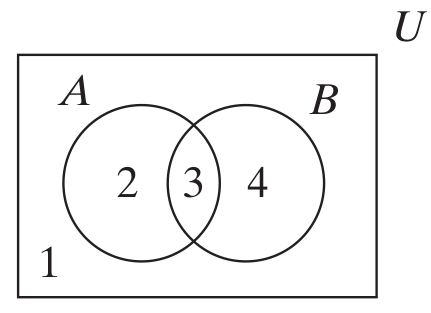
\includegraphics[scale=0.4]{images/diagram_venn}		
	\end{figure}
	\begin{itemize}
		\item<2-> In a Venn diagram, a rectangle depicts a universal set.
		\item<3-> Subsets of the universal set are drawn as circles.
		\item<4-> The inside of a circle represents the members of that set.
	\end{itemize}	
\end{frame}

\begin{frame}{Soal 2: Diagram Venn (2/2)}   
Di sebuah sekolah terdapat 4 klub. Berikut penjelasan anggota tiap klub.
\begin{itemize}
	\item Setiap siswa tergabung ke setidaknya satu klub.
	\item Setiap anggota klub $B$ adalah anggota klub $A$.
	\item Sebagian anggota klub $C$ adalah anggota klub $B$.
	\item Semua anggota klub $C$ yang merupakan anggota klub $A$ juga merupakan anggota klub $B$.
	\item Tidak ada anggota klub $D$ yang merupakan anggota klub $A$.
	\item Sebagian anggota klub $D$ adalah anggota klub $C$.
	\item Jumlah seluruh siswa adalah $140$.
	\item Jumlah anggota klub $A$ dan klub $C$ adalah $125$.
	\item Jumlah anggota klub $B$ adalah $40$.
	\item Jumlah anggota klub $D$ adalah $35$.
\end{itemize}
\onslide<2-> \textbf{Berapa jumlah siswa yang merupakan anggota di 1 klub saja?}
\end{frame}

\begin{frame}{Solusi (1/2)}
	\begin{figure}[!ht]
		\centering
		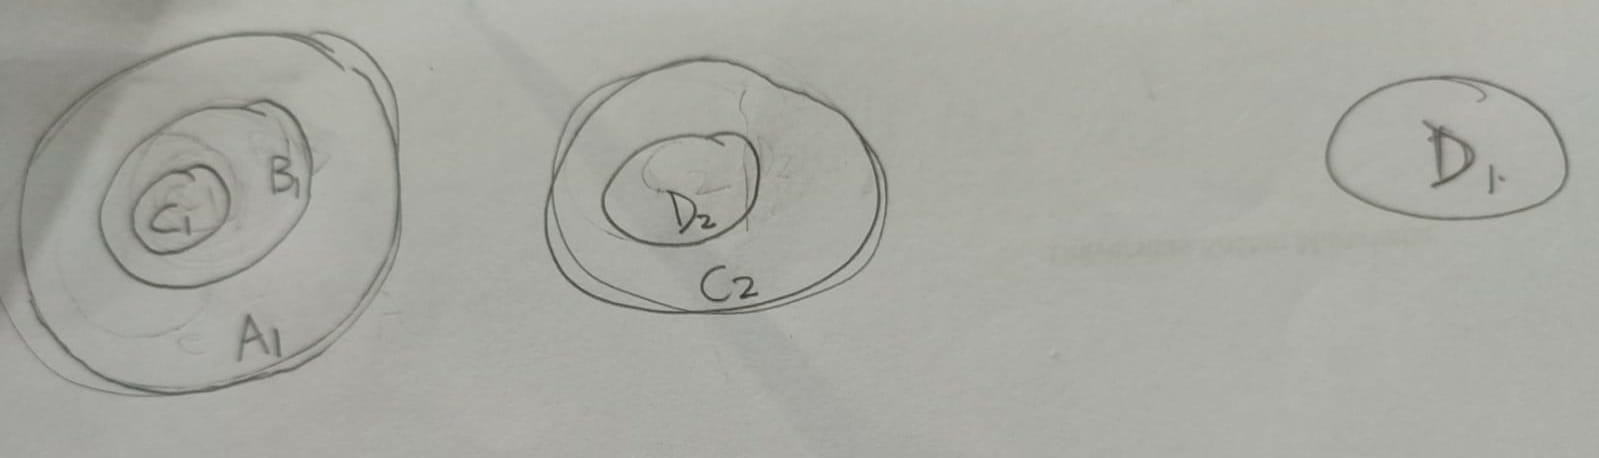
\includegraphics[scale=0.2]{images/solusi-soal-2}		
	\end{figure}
	Jumlah anggota klub $A$ dan $C$ adalah 125 $\Rightarrow$
	\begin{equation}
		A_1 + \underbrace{C_1 + B_1}_{\onslide<2->{\text{anggota klub }B}} + C_2 + D_2 = 125.
		\label{eq:A-dan-C}
	\end{equation}
	Jumlah anggota klub $B$ adalah 40 $\Rightarrow C_1 + B_1 = 40$. Oleh karenanya, Persamaan~(\ref{eq:A-dan-C}) menjadi 	
	\begin{equation}
		A_1 + 40 + C_2 + D_2 = 125.
		\label{eq:A-B-dan-C}
	\end{equation}
\end{frame}

\begin{frame}{Solusi (2/2)}
Jumlah seluruh siswa adalah 140 $\Rightarrow$
\begin{equation}
	A_1 + 40 + C_2 + D_2 + D_1 = 140.
	\label{eq:seluruh-siswa}
\end{equation}
Substitusi Persamaan~(\ref{eq:A-B-dan-C}) ke Persamaan~(\ref{eq:seluruh-siswa}) menjadi
\begin{equation}
	125 + D_1 = 140 \Longleftrightarrow D_1 = 15.
	\label{eq:d-1}
\end{equation}

Jumlah anggota kelas $D$ adalah 35, maka 
\begin{align}
	D_1 + D_2 = 35 \Longleftrightarrow 15 + D_2 = 35 \Longleftrightarrow D_2 = 20.
	\label{eq:d-2}
\end{align}

Substitusi Persamaan~\eqref{eq:d-2} ke Persamaan~\eqref{eq:seluruh-siswa} menjadi
\begin{align*}
	A_1 + 40 + C_2 + 20 + D_1 = 40 &\Leftrightarrow A_1 + C_2 + D_1 + 60 = 140 \\
	                               &\Leftrightarrow \underbrace{A_1 + C_2 + D_1}_{\text{Anggota di satu klub saja}} = 80. 
\end{align*}
Jadi jumlah siswa yang merupakan anggota di 1 klub saja adalah 80.
\end{frame}


\begin{frame}{Soal 3: Logika}
Ada 6 orang yaitu Albert, Budi, Caca, Danis, Eka, dan Farah, yang masing-masing mengeluarkan sebuah pernyataan yang hanya bisa bernilai benar atau salah saja.

\bigskip
\begin{tabular}{ll}
Albert (A) &: Pernyataanku bernilai benar \\
Budi (B)   &: Antara pernyataan Caca atau Albert \\
Caca (C)   &: Pernyataanku bernilai benar \\
Danis (D)  &: Pernyataan Budi bernilai benar \\
Eka (E)    &: Pernyataan Caca bernilai benar \\
Farah (F)  &: Pernyataanku bernilai benar
\end{tabular} 

\bigskip
Jika \textit{hanya ada tepat 1 pernyataan yang benar dari keenam pernyataan di atas}, pernyataan siapakah yang benar?
\end{frame}

\begin{frame}{Solusi}
\textbf{Skenario I:}\\
\begin{itemize}
	\item A benar
	\item B kudu salah $\Rightarrow$
	\begin{itemize}
		\item A salah \& C salah $\Rightarrow$ ngga mungkin 
		\item A benar \& C benar $\Rightarrow$ ngga bisa juga 
	\end{itemize}
\end{itemize}

\textbf{Skenario II:}\\
\begin{itemize}
	\item A salah
	\item B benar
	\item C benar $\Rightarrow$ ngga bisa!
\end{itemize}

\textbf{Skenario III:}\\
\begin{itemize}
	\item A salah
	\item B salah
	\item C salah
	\item D salah
	\item E salah
	\item \textbf{F benar} $\Rightarrow$ Jadi pernyataan \textbf{Farah} yang benar.
\end{itemize}
\end{frame}

\begin{frame}{Soal 4: Analisis Kemungkinan dengan Logika (1/)}
Tabel Kebenaran untuk \textit{Jika-Maka}.

\begin{table}[!ht]
\centering
\begin{tabular}{|c|c|c|}
\hline
$\bm{p}$ & $\bm{q}$ & $\bm{p \longrightarrow q}$ \\
\hline
True  & True & True \\
\hline
True  & False & False \\
\hline
False & True & True \\
\hline
False & False & True \\
\hline
\end{tabular}
\end{table}

Tabel Kebenaran untuk \textit{Exclusive-OR}.

\begin{table}[!ht]
\centering
\begin{tabular}{|c|c|c|}
\hline
$\bm{p}$ & $\bm{q}$ & $\bm{p \oplus q}$ \\
\hline
True  & True & False \\
\hline
True  & False & True \\
\hline
False & True & True \\
\hline
False & False & False \\
\hline
\end{tabular}
\end{table}

Kontrapositif (\textit{Contrapositive}) adalah
\begin{equation*}
p \longrightarrow q \Longleftrightarrow \text{ NOT }q \longrightarrow \text{ NOT }q
\end{equation*}
\end{frame}

\begin{frame}{Soal 4: Analisis Kemungkinan dengan Logika (2/)}
Empat orang sekawan yaitu Kwak, Kwik, Kwek, dan Kwok akan berlibur ke kota Bandung. Akan tetapi karena satu dan lain hal, beberapa (bisa saja tidak ada) dari mereka gagal untuk berlibur ke Kota Bandung. Mereka akhirnya menetapkan aturan berikut untuk menentukan siapa yang akan berlibur ke Kota Bandung

\begin{itemize}
	\item Jika Kwak pergi ke Bandung maka Kwik juga akan ikut ke Bandung.
	\item Hanya tepat salah satu dari Kwik atau Kwek yang akan pergi ke Bandung.
	\item Jika Kwek pergi ke Bandung maka Kwak dan Kwok keduanya harus pergi ke Bandung.
	\item Jika Kwok tidak pergi ke Bandung, maka Kwik juga tidak akan pergi ke Bandung.
\end{itemize}

Berapa banyak kemungkinan orang-orang yang akan pergi ke Bandung?
\end{frame}

\begin{frame}{Solusi (1/2)}
Kwak = Kwak pergi, Kwik = Kwik pergi, Kwek = Kwek pergi, dan Kwok = Kwok pergi.
\begin{enumerate}
	\item Kwak $\longrightarrow$ Kwik 
	\item Kwik $\oplus$ Kwek
	\item Kwek $\longrightarrow$ Kwak AND Kwok 
	\item NOT Kwok $\longrightarrow$ NOT Kwik.
\end{enumerate}

Kuncinya adalah \textbf{poin 2}, yaitu (Kwik pergi) $\oplus$ (Kwek pergi).

\begin{table}[!ht]
	\centering
	\caption{Ketika Kwik pergi}
	\begin{tabular}{|cc|cc|}
		\hline
		Kwak & \cmark & Kwak & \xmark \\
		\hline 	
		Kwik & \cmark & Kwik & \cmark \\
		\hline
		Kwek & \xmark & Kwek & \xmark \\
		\hline
		Kwok & \cmark & Kwok & \cmark \\
		\hline		
	\end{tabular}
\end{table}  
\end{frame}

\begin{frame}{Solusi (2/2)}
\begin{table}[!ht]
	\centering
	\caption{Ketika Kwek pergi $\Rightarrow$ Kontradiksi untuk Kwak}
	\begin{tabular}{|cc|}
		\hline
		Kwak  & \xmark \\
		\hline 	
		Kwik & \xmark  \\
		\hline
		Kwek & \cmark  \\
		\hline
		Kwok & \cmark  \\
		\hline		
	\end{tabular}
\end{table}  
Jadi hanya ada 2 kemungkinan, yaitu:
\begin{table}[!ht]
	\centering
	\begin{tabular}{|cc|cc|}
		\hline
		Kwak & \cmark & Kwak & \xmark \\
		\hline 	
		Kwik & \cmark & Kwik & \cmark \\
		\hline
		Kwek & \xmark & Kwek & \xmark \\
		\hline
		Kwok & \cmark & Kwok & \cmark \\
		\hline		
	\end{tabular}
\end{table}  
\end{frame}

\begin{frame}{Soal 5: Operasi Logika}
Perhatikan operasi logika berikut!
\begin{align*}
P &= (A \text{ AND }(\text{NOT }B)) \text{ OR }((C \text{ OR }(\text{ NOT }D)) \text{ AND } (\text{ NOT }E)) \\
Q &= ((\text{NOT }A) \text{ OR }(\text{NOT }B)) \text{ AND }(((\text{NOT }C) \text{ AND }D) \text{ OR }(\text{NOT } E))  \\
R &= P \text{ AND }Q.
\end{align*}
Jika $A$ = True, $B$ = True, $C$ = True, $D$ = True, dan $E$ = False. Tentukan nilai $P$, $Q$, dan $R$ berturut-turut?
\end{frame}

\begin{frame}{Solusi}
Silakan adik-adik untuk mencobanya sendiri ya. 

\bigskip
Jawaban yang saya peroleh adalah
\begin{align*}
P &= \text{True} \\
Q &= \text{False} \\
R &= \text{False}. 
\end{align*}
\end{frame}

\begin{frame}{Soal 6: Keliling Terkecil}
Pak Dengklek memiliki 8 titik yang terletak pada koordinat:
\begin{equation*}
(2,5), (3,8), (3,4), (4,8), (4,0), (3,3), (0,4), (0,0)
\end{equation*}
Beliau ingin menutupi kedelapan titik tersebut dengan sebuah poligon sedemikian sehingga setiap titik milik Pak Dengklek berada di dalam (atau di tepi) poligon tersebut. 

\bigskip
Berapa \textit{keliling poligon terkecil} yang memenuhi keinginan Pak Dengklek?
\end{frame}

\begin{frame}{Solusi}
\begin{figure}[!ht]
	\centering
	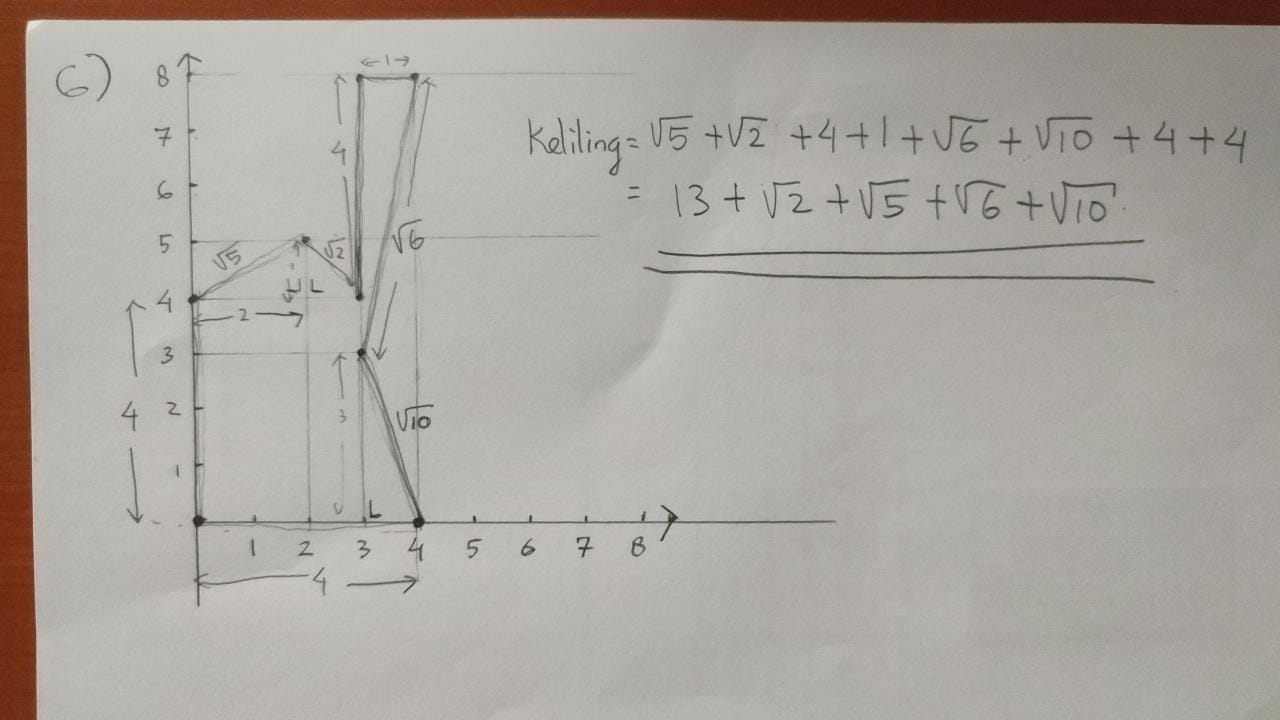
\includegraphics[scale=.26]{images/solusi-soal-6}
	\caption{Bentuk poligon yang ditulis dengan tulisan tangan}
\end{figure}

\end{frame}

\begin{frame}{Soal 7: Dijkstra's Algorithm (1/)} 
Kerajaan Zidan sedang berperang melawan Kerajaan Ahmad. Salah satu mata-mata Kerajaan Zidan berhasil mendapatkan peta logistik Kerajaan Ahmad, yaitu sebagai berikut:
\begin{figure}[!ht]
	\centering
	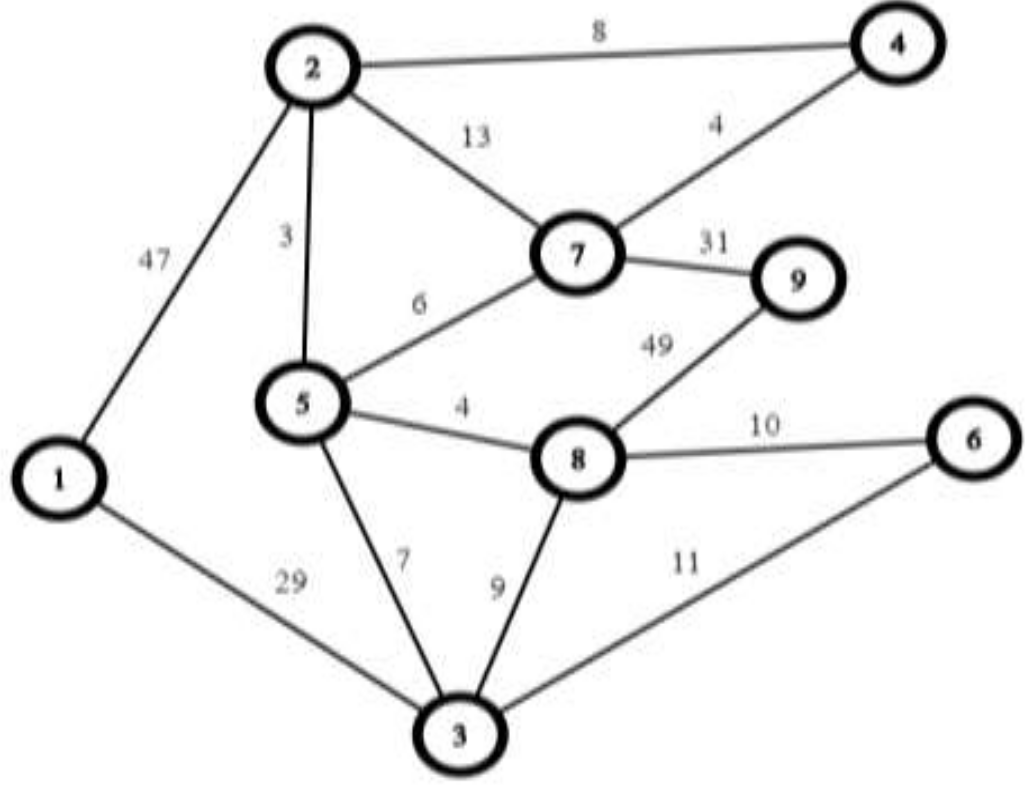
\includegraphics[scale=.225]{images/soal-7-peta}
\end{figure}
\end{frame}

\begin{frame}{Soal 7: Dijkstra's Algorithm (2/)} 
Sumber logistik Kerajaan Ahmad berada di node bernomor 1 dan Kerajaan Ahmad berada di node bernomor 9. Kerajaan Zidan ingin memutus jalur logistik Kerajaan Ahmad agar memenangkan perang. Dengan kata lain, Kerajaan Zidan ingin menghancurkan beberapa jalan sedemikian sehingga tidak ada jalan yang bisa digunakan untuk mencapai node 9 dari node 1, dan sebaliknya. Bilangan yang tertera pada jalan merupakan biaya yang dibutuhkan Kerajaan Zidan untuk menghancurkan jalan tersebut. 

\bigskip
\textit{Berapa total biaya minimum yang dibutuhkan Kerajaan Zidan?}
\end{frame}

\begin{frame}{Solusi~\citep{epp2020discrete}}
\begin{figure}[!ht]
	\centering
	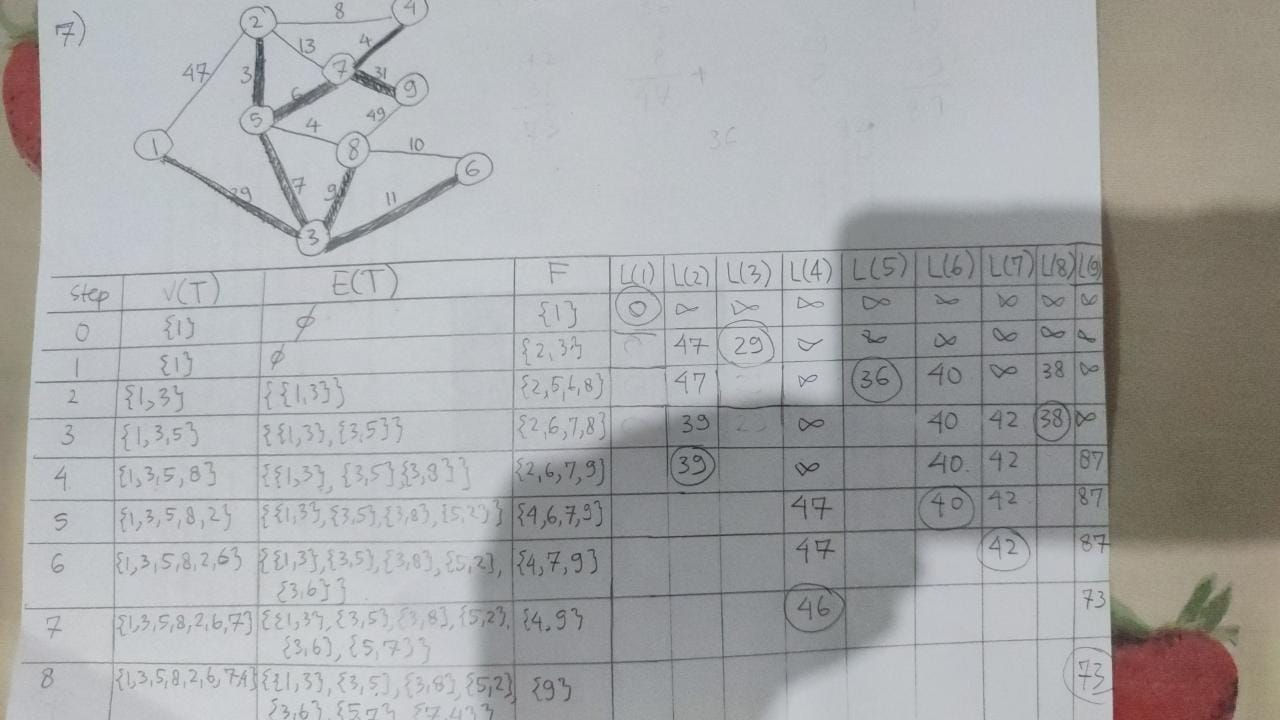
\includegraphics[scale=.275]{images/solusi-soal-7}
\end{figure}
\end{frame}

\begin{frame}{Soal 8: Permutasi}
Terdapat 4 ekor bebek berwarna merah, 3 ekor bebek berwarna biru, dan 2 ekor bebek berwarna hijau. Kesembilan bebek tersebut diminta untuk berbaris oleh Pak Dengklek dengan ketentuan:

\begin{itemize}
	\item Setiap bebek yang berwarna sama tidak bisa dibedakan.
	\item Untuk setiap pasang bebek yang berwarna sama, tidak boleh ada bebek lain yang warnanya berbeda yang berada di antara sepasang bebek tersebut.
\end{itemize}

\bigskip
\textit{Ada berapa macam posisikah yang mungkin dalam barisan bebek tersebut?}
\end{frame}

\begin{frame}{Solusi}
Jawab: 
\begin{align*}
	3! &= 3 \times 2 \times 1 \\
	   &= 6.
\end{align*}
\end{frame}

\begin{frame}{Soal 9: Teknik Analisis Rekursif}
Pak Dengklek memiliki sebuah fungsi $f$ yang dapat dinyatakan sebagai berikut:
\begin{equation*}
f(z) =
\left\{ \begin{array}{rcl}
1                       & \mbox{for} & n \leq 1 \\ 
f(\frac{n}{2}) * 2 + n, & \mbox{for} & n > 1
\end{array}\right.
\end{equation*}
Berapakah nilai $f(1048576)$?
\end{frame}

\begin{frame}{Solusi (1/2)~\citep{levitin2012introduction}}
Misalkan $n=2^k$ maka $k = \log_2 n$ kemudian
\begin{equation*}
f(2^k) = f(2^{k-1}) * 2 + 2^k, \; \text{ untuk } 2^k > 1.
\end{equation*}
Selanjutnya,
\begin{align*}
	f(2^k) &= f(2^{k-1}) * 2 + 2^k \\
	       &= (f(2^{k-2}) * 2 + 2^{k-1}) * 2 + 2^k  \\
	       &= f(2^{k-2}) * 2^2 + 2^k + 2^k \\
	       &= (f(2^{k-3}) * 2 + 2^{k-2}) * 2^2 + 2^k + 2^k \\
	       &= f(2^{k-3}) * 2^3 + 2^k + 2^k + 2^k \\
	       &= (f(2^{k-4}) *2 + 2^{k-3}) * 2^3 + 2^k + 2^k + 2^k \\
	       &= f(2^{k-4}) * 2^4 + 2^k + 2^k + 2^k + 2^k \\
	       &= f(2^{k-j}) * 2^j + j * (2^k).
\end{align*}
\end{frame}

\begin{frame}{Solusi (2/2)}
Kita peroleh
\begin{equation*}
	f(2^k) = f(2^{k-j}) * 2^j + j * (2^k).
\end{equation*}

Pilih $j=k$,
\begin{align*}
	f(2^k) &= f(2^0) * 2^k + (k) * 2^k \\
	       &= 2^k + k * 2^k \\
	       &= 2^k * (1+k) \\
	       &= n * (1 + \log_2 n) && \text{dengan }n=2^k \text{ dan }k=\log_2 n.
\end{align*}

Jadi 
\begin{equation*}
f(n) = n * (1 + \log_2 n)
\end{equation*}
dan
\begin{equation*}
f(1048576) = 1048576 * (1 + \log_2 1048576).
\end{equation*}
\end{frame}

\begin{frame}{Soal 10: Dynamic Programming}
Pak Dengklek memiliki sebuah sekuens $S = \{2, 14, 7, 20, 5, 3, 8, 11, 18, 4, 10, 12, 1, 6, 9, 19, 15, 16, 13, 17\}$. \\
Subsekuens dari sebuah sekuens $S$ bisa didapatkan dengan menghilangkan beberapa elemen dari $S$ namun dengan tetap mempertahankan urutannya. Sebagai Contoh: $\{2, 7, 13, 17\}$ adalah subsekuens dari $S$, sedangkan $\{14, 2, 20\}$ bukanlah subsekuens dari $S$ karena urutannya berubah (2 muncul lebih dahulu dari 14 di $S$).

\bigskip
Pak Dengklek ingin mencari sebuah subsekuens menaik dari $S$. Sebuah subsekuens dikatakan menaik jika dan hanya jika elemen-elemen yang ada di dalam subsekuens tersebut tersusun secara menaik. Sebagai Contoh: $\{2, 7, 20\}$. 

\bigskip
Berapa banyaknya elemen dari subsekuens menaik terpanjang yang bisa dibentuk dari sekuens $S$?
\end{frame}

\begin{frame}{Solusi}
\begin{figure}[!ht]
\centering
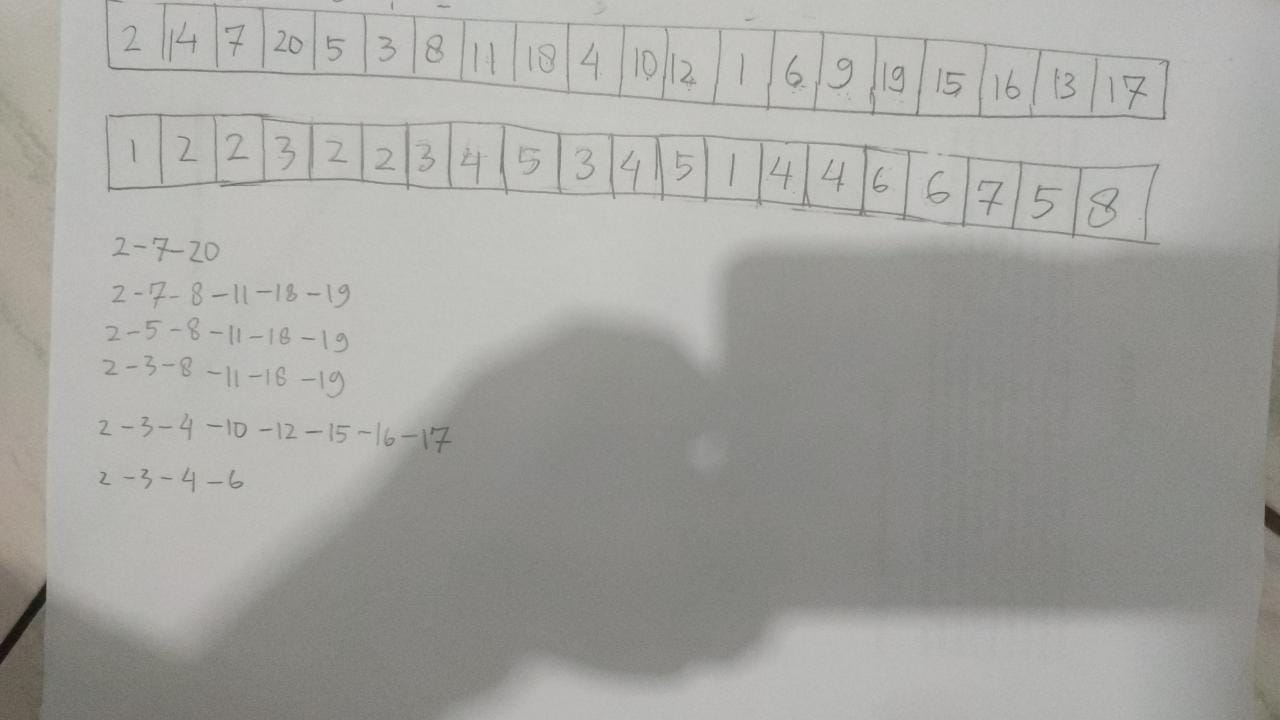
\includegraphics[scale=.25]{images/solusi-soal-10}
\end{figure}
\end{frame}


%%%% predictive distribution


 % \begin{frame}
 %   \frametitle{Some other one parameter models}

 %   \begin{itemize}
 %   \item Poisson
 %   \item Exponential
 %   \item Cauchy
 %   \end{itemize}
   
 % \end{frame}

\section<presentation>*{\appendixname}
\subsection<presentation>*{For Further Reading}

\begin{frame}[allowframebreaks]
  \frametitle<presentation>{Daftar Pustaka}
    {\footnotesize
%    \bibliographystyle{apalike}
    \bibliography{references}
    }    
\end{frame}

\end{document}

%%% Local Variables: 
%%% TeX-PDF-mode: t
%%% TeX-master: t
%%% End: 
